% CVPR 2022 Paper Template
% based on the CVPR template provided by Ming-Ming Cheng (https://github.com/MCG-NKU/CVPR_Template)
% modified and extended by Stefan Roth (stefan.roth@NOSPAMtu-darmstadt.de)

\documentclass[10pt,twocolumn,letterpaper]{article}

%%%%%%%%% PAPER TYPE  - PLEASE UPDATE FOR FINAL VERSION
\usepackage[review]{cvpr}      % To produce the REVIEW version
%\usepackage{cvpr}              % To produce the CAMERA-READY version
%\usepackage[pagenumbers]{cvpr} % To force page numbers, e.g. for an arXiv version

% Include other packages here, before hyperref.
\usepackage{graphicx}
\usepackage{amsmath}
\usepackage{amssymb}
\usepackage{booktabs}
\usepackage{enumitem}
\usepackage{float}

% It is strongly recommended to use hyperref, especially for the review version.
% hyperref with option pagebackref eases the reviewers' job.
% Please disable hyperref *only* if you encounter grave issues, e.g. with the
% file validation for the camera-ready version.
%
% If you comment hyperref and then uncomment it, you should delete
% ReviewTempalte.aux before re-running LaTeX.
% (Or just hit 'q' on the first LaTeX run, let it finish, and you
%  should be clear).
\usepackage[pagebackref,breaklinks,colorlinks]{hyperref}


% Support for easy cross-referencing
\usepackage[capitalize]{cleveref}
\crefname{section}{Sec.}{Secs.}
\Crefname{section}{Section}{Sections}
\Crefname{table}{Table}{Tables}
\crefname{table}{Tab.}{Tabs.}


%%%%%%%%% PAPER ID  - PLEASE UPDATE
\def\cvprPaperID{47} % *** Enter the CVPR Paper ID here
\def\confName{AI2100}
\def\confYear{2022}


\begin{document}

%%%%%%%%% TITLE - PLEASE UPDATE
\title{Explaining answers given by neural question answering systems}
\maketitle

%%%%%%%%% ABSTRACT
\begin{abstract}
Question answering has been a fundamental challenge in NLP with vast applications. State of the art neural question answering systems are able to beat humans at this task when evaluated on carefully prepared datasets. However it is difficult to explain in human comprehensible manner, how these models reach the answers that they do. Such an explanation is often important in high stakes situations such as healthcare or business applications. Hence, we explored various explainability methods in the context of neural question answering through this project and verified some of their results. We also report our findings and frame adversarial examples to support our claims.
\end{abstract}

%%%%%%%%% BODY TEXT
\section{Approach}
We analysed BERT model for the task of RCQA using integrated gradients. We fine tuned BERT-base-uncased for 3 epochs on SQuAD-v1 and saved the fine-tuned model. To understand what the fine-tuned BERT is looking at, and to explain the functionality of its layers, we propose to use the embeddings that are produced after each layer. A few previous works look at attention scores produced by BERT to conclude facts about interpretability. But, more recent work \cite{at_not_exp} shows that attention, atleast in some cases, is not suited for explainability. Hence we chose to work on the embeddings which carry some information about what BERT has learnt, from each layer. We analyse them using two approaches:
\begin{enumerate}
    \item Visualisations of integrated gradients of embeddings, after each layer
    \item t-SNE visualisations of the embeddings, after each layer.
\end{enumerate}
In the following section, we verify the results which previous works have found. Also, we outline some of our findings for the fine tuned model. Using Integrated gradient technique, we came to the conclusion that Bert model uses certain heuristics to answer question. To further verify this claim, we built adversarial examples on which these heuristics would not work. We found that Bert model did fail on these adversarial examples.

\section{Results}
\subsection{Verification of some of the previous works}
\begin{enumerate}
    \item \cite{bert_for_qa} claims that initial layers of BERT focus on question words in the passage. In the later layers, the focus on question words decreases, and more focus is on supporting words that surround the answer. Their approach uses Integrated Gradients. Proceeding on similar lines, we confirm their claims.
\end{enumerate}

We calculated the attribution scores for embeddings of words after each layer using integrated gradients approach. We leveraged the captum library to achieve this. We visualised these using the inbuilt-captum functionality, as well as by plotting the heatmaps. \\\\Consider the context-question pair given below.\\
\textbf{Context: }The Panthers finished the regular season with a 15–1 record, and quarterback Cam Newton was named the NFL Most Valuable Player (MVP). They defeated the Arizona Cardinals 49–15 in the NFC Championship Game and advanced to their second Super Bowl appearance since the franchise was founded in 1995. The Broncos finished the regular season with a 12–4 record, and denied the New England Patriots a chance to defend their title from Super Bowl XLIX by defeating them 20–18 in the AFC Championship Game. They joined the Patriots, Dallas Cowboys, and Pittsburgh Steelers as one of four teams that have made eight appearances in the Super Bowl. The 2020 regular season win/loss ratio for the Michigan Vikings was 656.\\
\textbf{Question: }How many appearances have the Broncos made in the super bowl?\\
\textbf{Predicted Answer: }eight\\
% The following are the visual
% \onecolumn
% \begin{figure}[!htp]
%     \centering
%     \begin{subfigure}[t]{\columnwidth}
%     \centering
%     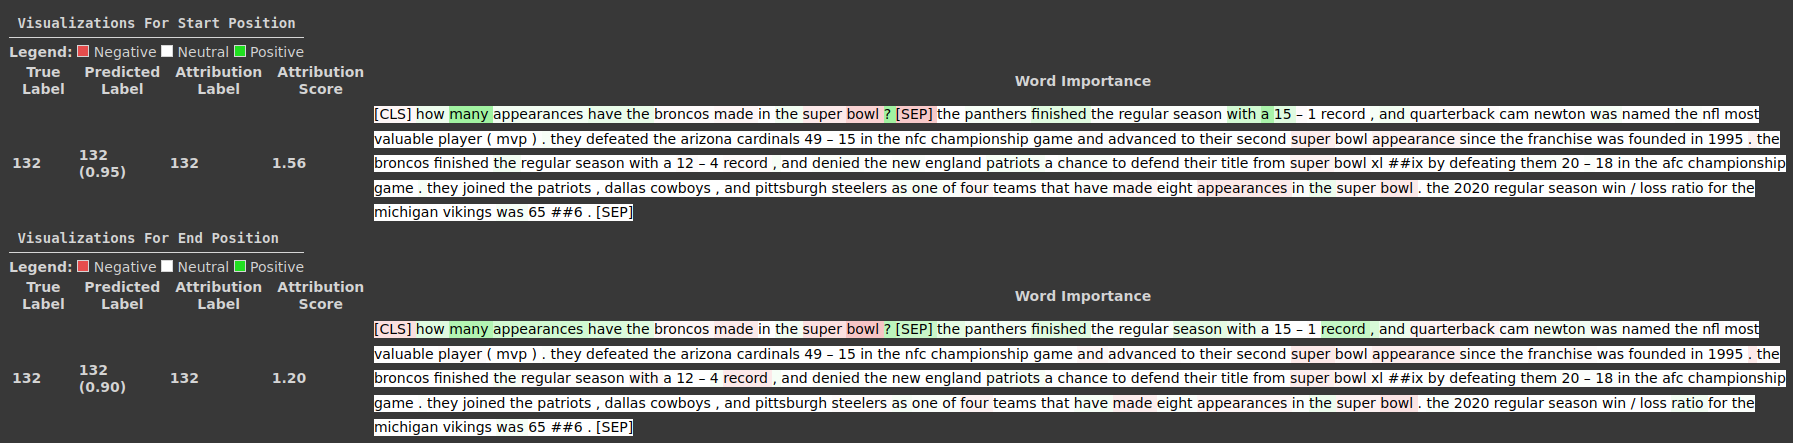
\includegraphics[width=\linewidth]{ll0.png}
%     \end{subfigure}
%     \begin{subfigure}[t]{\columnwidth}
%     \centering
%     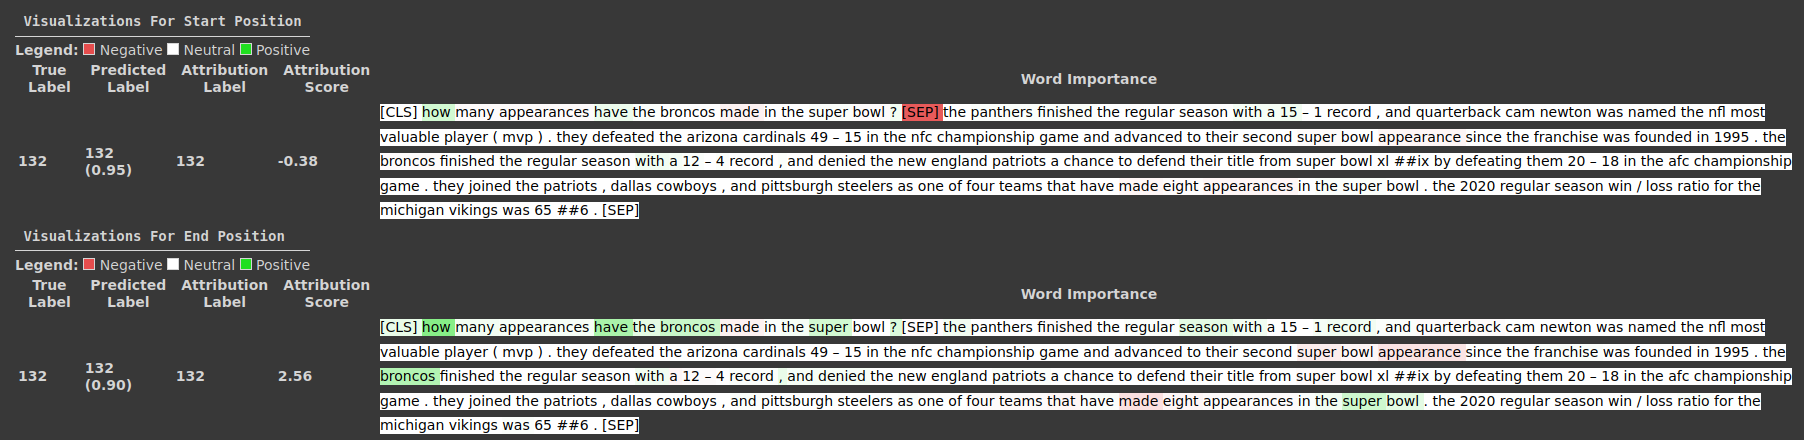
\includegraphics[width=\linewidth]{ll1.png}
%     \end{subfigure}
%     \begin{subfigure}[t]{\columnwidth}
%     \centering
%     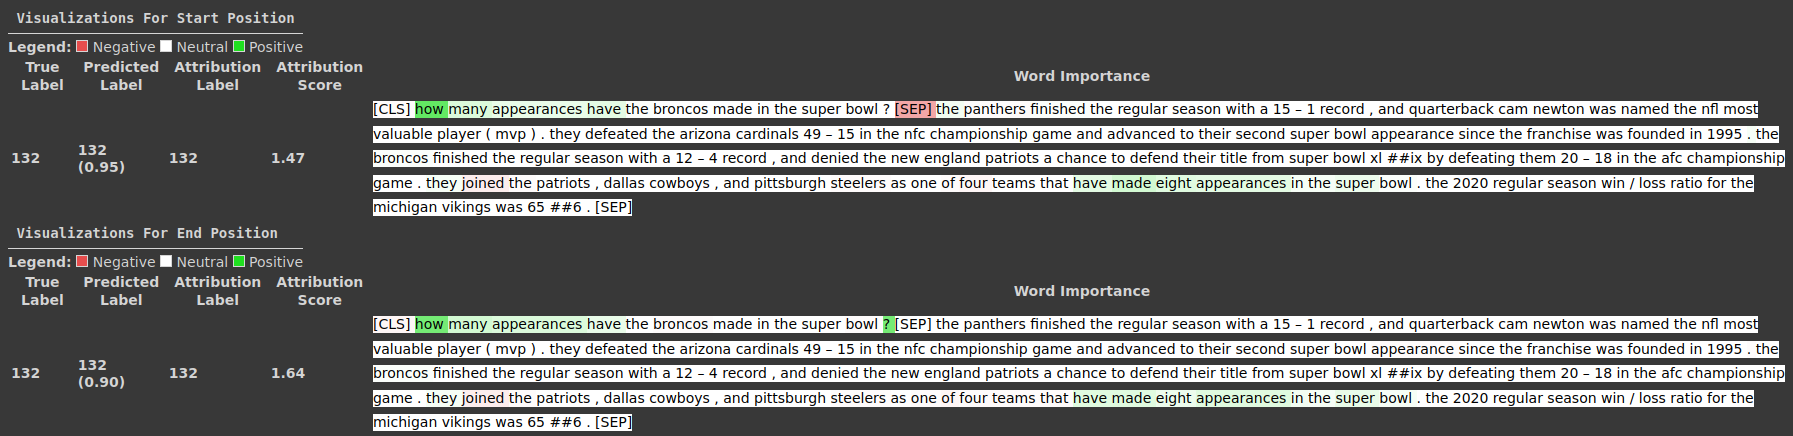
\includegraphics[width=\linewidth]{ll5.png}
%     \end{subfigure}
%     \begin{subfigure}[t]{\columnwidth}
%     \centering
%     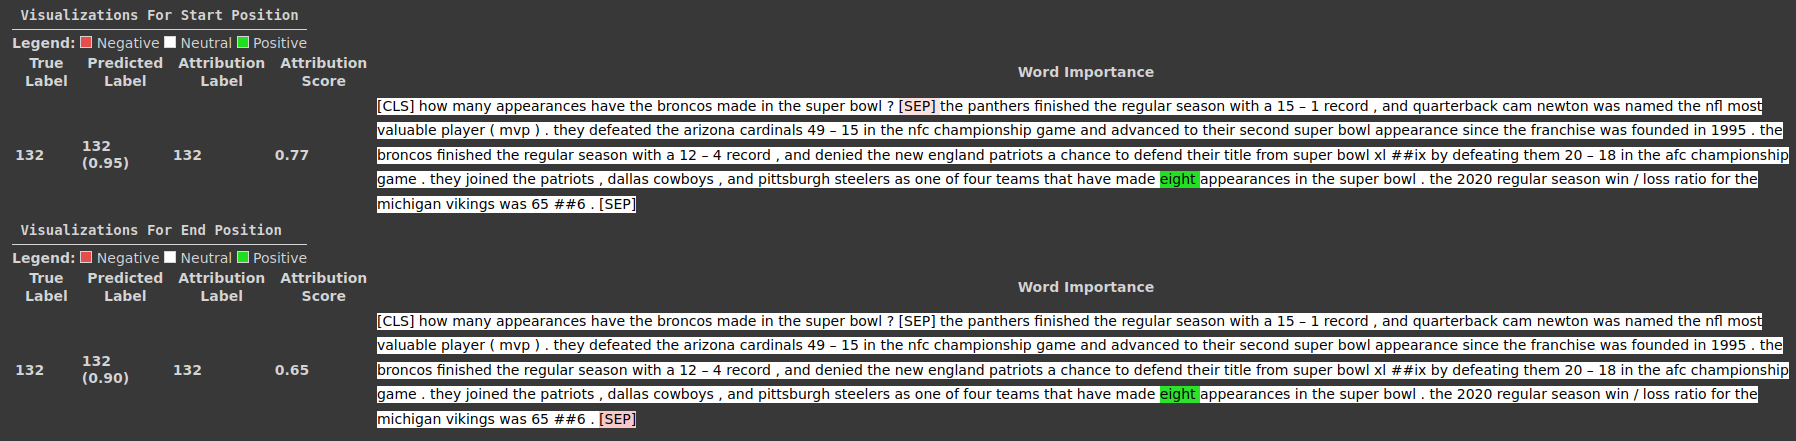
\includegraphics[width=\linewidth]{ll11.png}
%     \end{subfigure}
%     \caption{t-SNE visualisations of word embeddings after a layer.}
%     \label{fig:plot1}
% \end{figure}
% \twocolumn

We use captum library to plot our results. We indeed get similar results \ref{fig:plot1} which the paper claims. Initial layers focus more on question words in context. Later layers, try to look at supporting context words. Finally, the model focuses on the answer in the last layers.
\begin{enumerate}[resume]
    \item \cite{bert_layers_qa} claims that initial layers look at the semantic meanings of each word, and subsequent layers look at relations between the words in context. The final layers filter out the relevant information, and come up with the answer. Their approach uses PCA visualisation of embeddings.  Proceeding on similar lines, we confirm their claims.
\end{enumerate}
Consider the context-question pair given below.\\
\textbf{Context: }Alfred is a white cat and likes apples. Bobby is a black dog which loves mangoes.\\
\textbf{Question: }What does Alfred like?\\
\textbf{Predicted Answer: }Apples
\\\\
We perform t-SNE visualisations of embeddings after each layer, instead of PCA, in order to preserve more information, which might have possibly lost during PCA. We indeed get similar results \ref{fig:plot2} which the paper claims.
\begin{figure}[!htp]
    \centering
    \begin{subfigure}[t]{0.65\columnwidth}
    \centering
    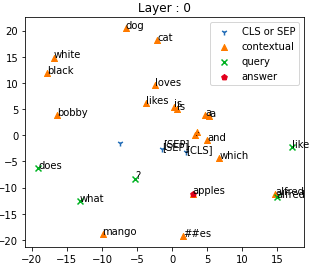
\includegraphics[width=\linewidth]{l0.png}
    \end{subfigure}
    \begin{subfigure}[t]{0.65\columnwidth}
    \centering
    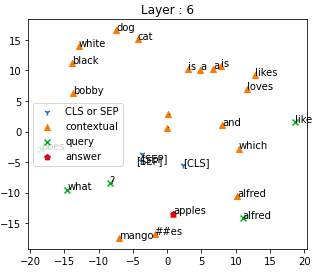
\includegraphics[width=\linewidth]{l6.png}
    \end{subfigure}
    \begin{subfigure}[t]{0.65\columnwidth}
    \centering
    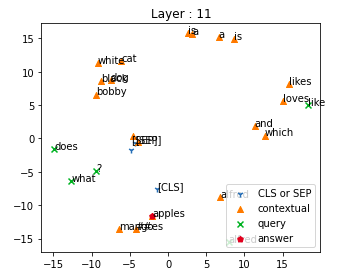
\includegraphics[width=\linewidth]{l11.png}
    \end{subfigure}
    \caption{t-SNE visualisations of word embeddings after a layer.}
    \label{fig:plot2}
\end{figure}
Initial layers look at semantic meanings of words (words like white, black or loves, like, or cat, dog occur together). Later layers, learn relations in context (white, cat, black, dog become together). Finally, all the important information is filtered out (apples, is reasonably seperated). 
% \begin{enumerate}[resume]
%     \item \cite{bert_for_qa} claims that BERT focuses on confusing words in later layers, rather than initial layers, and state an example context, question pair. However, we don't comment on the validity of their claim, as they do a qualitative analysis to back their results, which we are not able to reproduce due to lack of adequate information. We only point out an example which they described, and show its wrong.
% \end{enumerate}
% Consider the context-question pair given below.\\
% \textbf{Context: }The Panthers finished the regular season with a 15–1 record, and quarterback Cam Newton was named the NFL Most Valuable Player (MVP). They defeated the Arizona Cardinals 49–15 in the NFC Championship Game and advanced to their second Super Bowl appearance since the franchise was founded in 1995. The Broncos finished the regular season with a 12–4 record, and denied the New England Patriots a chance to defend their title from Super Bowl XLIX by defeating them 20–18 in the AFC Championship Game. They joined the Patriots, Dallas Cowboys, and Pittsburgh Steelers as one of four teams that have made eight appearances in the Super Bowl. The 2020 regular season win/loss ratio for the Michigan Vikings was 656.\\
% \textbf{Question:} How many appearances have the Broncos made in the super bowl?\\
% \textbf{Predicted Answer:} eight\\
% \ref{neg_10} and \ref{neg_11} show the visualisations of attributions for 

% \begin{figure}
%     \centering
%     \begin{subfigure}
%     \centering
%     \includegraphics[scale = 0.25]{layer10.png}
%     \caption{Attribution score visualisation for Layer 10}
%     \label{neg_10}
%     \end{subfigure}
%     \begin{subfigure}
%     \centering
%     \onecolumn\includegraphics[scale=0.25]{layer11.png}
%     \caption{Attribution score visualisation for Layer 11}
%     \label{neg_11}
%     \end{subfigure}
% \end{figure}
% \twocolumn

\subsection{Some of our (interesting) findings}
Analysing the heat-maps for different examples, we observed few patterns. First was that initially the model was focusing greatly on question words like "Who, What, When, Where". The model was also focusing on possible answers to such nouns and numbers in the query.
% For example, the following question and context pair gave figure \ref{ex1}\\
\\\\Consider the context-question pair given below \ref{ex1}\\
\textbf{Context: }93 players have been awarded the Fewest Prized Team distinction for the Champ Bowl.\\
\textbf{Question: }How many players have been awarded the Fewest Prized Team distinction for the Super Bowl?\\

Second was that as mentioned previously, the model was focusing on words which were same in the question and the context. Then the model was looking at neighbours of the words it focused on initially, as mentioned above. (Look at section 2.1).

Based on these observations, we claim that the Bert model uses heuristics to predict the start and end tokens. These heuristics work as follows:

\begin{enumerate}
    \item Recognize the question type by focusing on the question words. Focus on candidate answers.
    \item Focus on words that are same in both the question and the answer.
    \item Look at neighbouring words of the words on which we focused in the above steps and predict start and end tokens from these.
\end{enumerate}

How exactly the model picks start and end token during heuristic 3 is still a mystery.
\subsection{Verification of the claims using adversarial examples}
We constructed adversarial examples by assuming that the model uses these heuristics. We expected that the model to fail on these examples and that is exactly what happened.

To test heuristic 1, consider the context-question pair given below\\
\textbf{Context: }Yes, a person can jump from a hill and still be alive.\\
\textbf{Question: }After jumping from a hill, can a person be alive?\\
\textbf{Predicted Answer: }still be alive 
\onecolumn
\begin{figure}
    \centering
    \begin{subfigure}[t]{0.9\columnwidth}
    \centering
    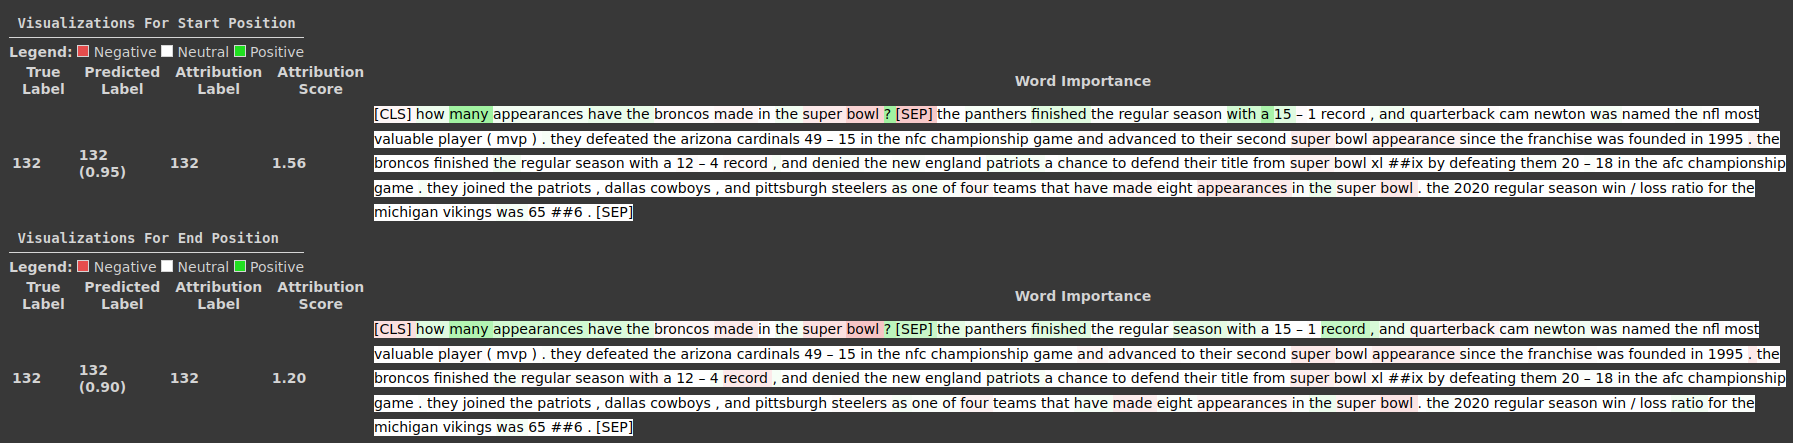
\includegraphics[width=\linewidth]{ll0.png}
    \end{subfigure}
    \begin{subfigure}[t]{0.9\columnwidth}
    \centering
    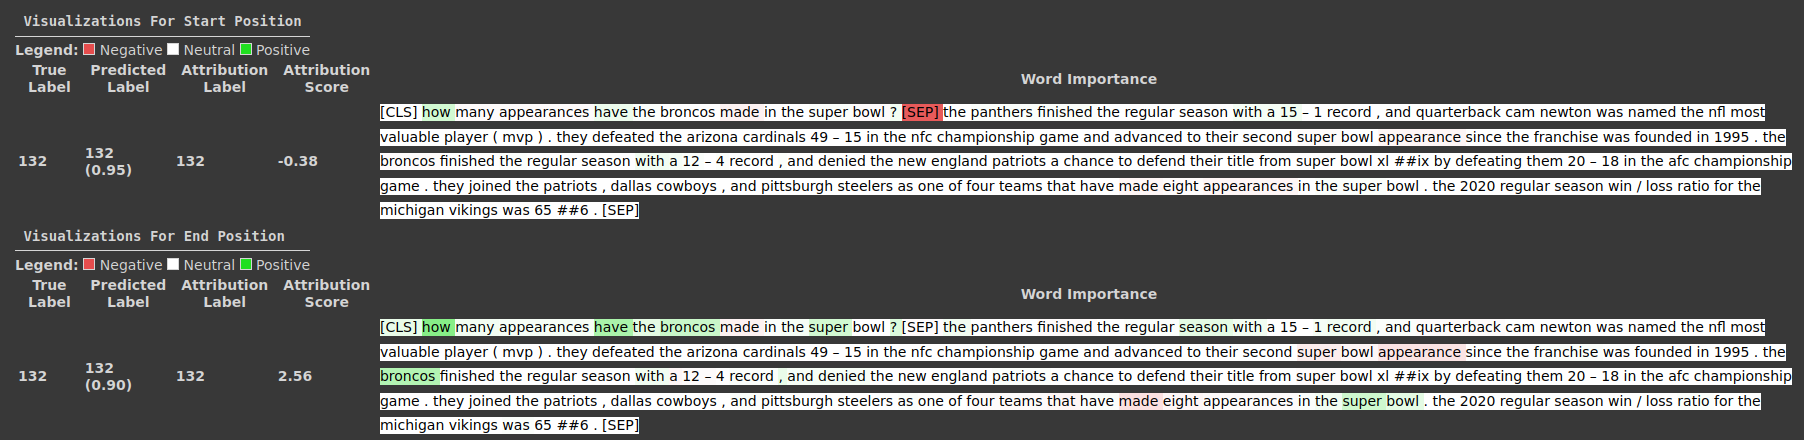
\includegraphics[width=\linewidth]{ll1.png}
    \end{subfigure}
    \begin{subfigure}[t]{0.9\columnwidth}
    \centering
    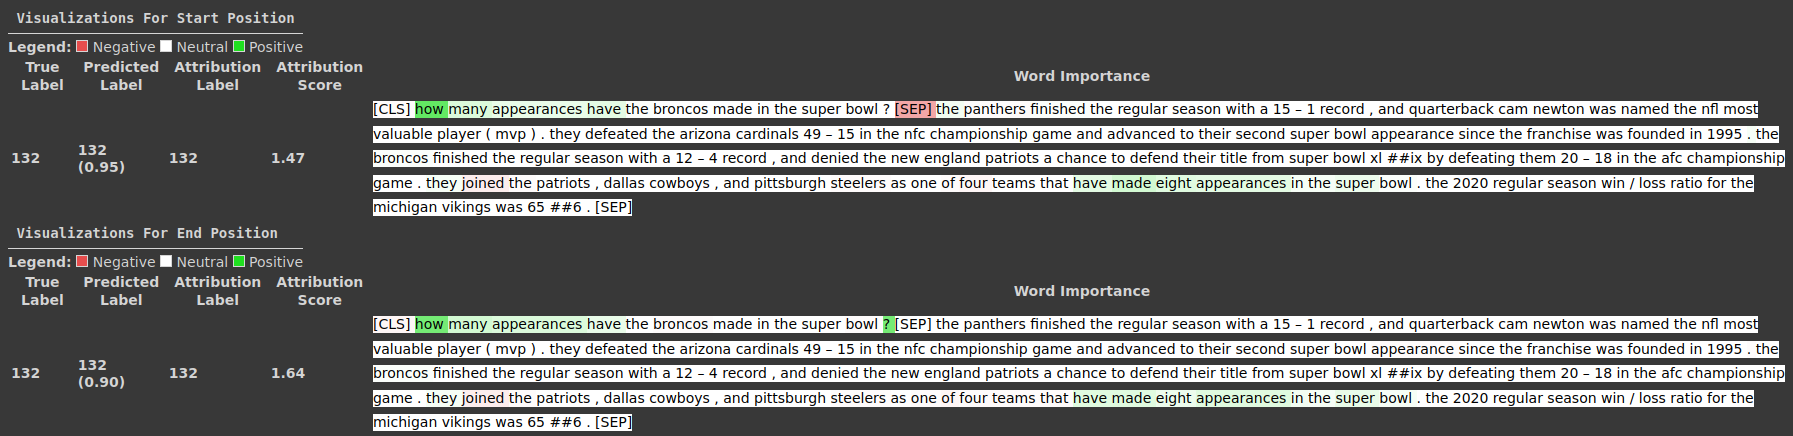
\includegraphics[width=\linewidth]{ll5.png}
    \end{subfigure}
    \begin{subfigure}[t]{0.9\columnwidth}
    \centering
    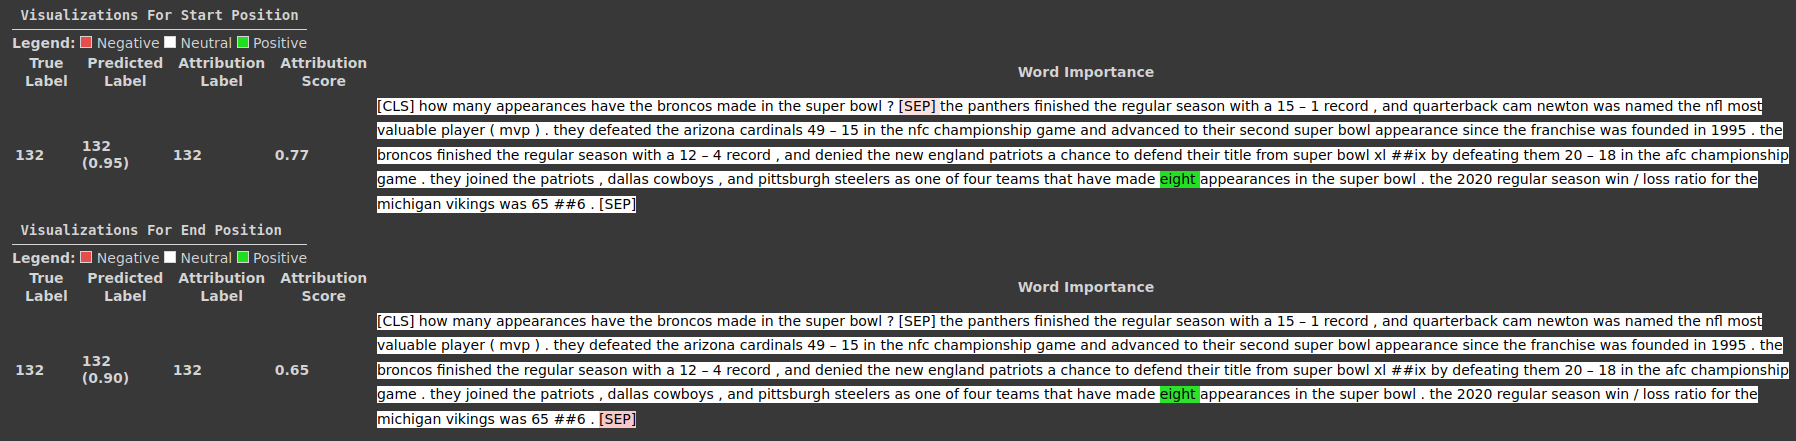
\includegraphics[width=\linewidth]{ll11.png}
    \end{subfigure}
    \caption{Visualisation of Integrated gradients of word embedding after a layer.}
    \label{fig:plot1}
\end{figure}
\twocolumn

\newpage
\onecolumn
\begin{figure}
    \onecolumn\centering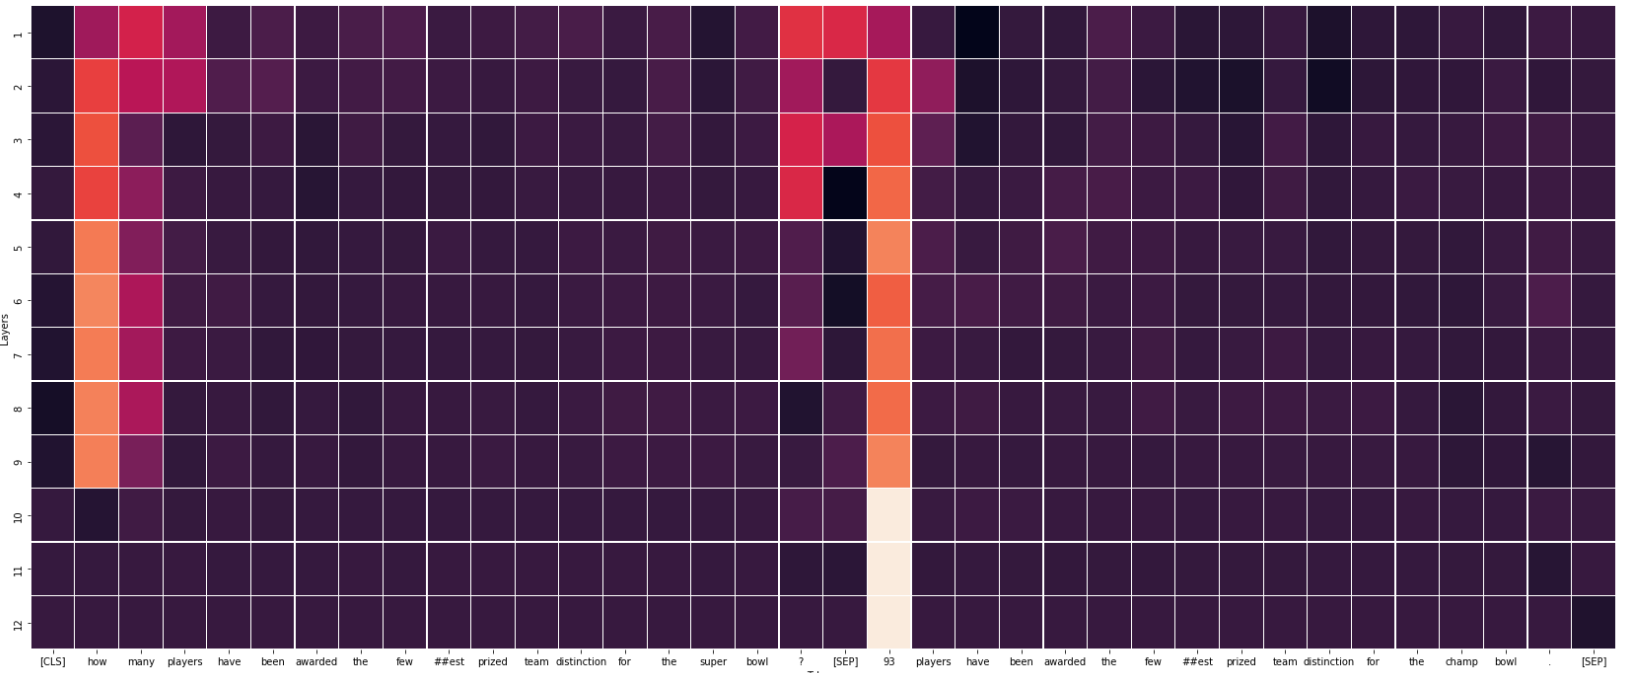
\includegraphics[scale=0.3]{obs1.png}
    \caption{Example demonstrating importance in initial layers}
    \label{ex1}
\end{figure}
\begin{figure}
    \centering
    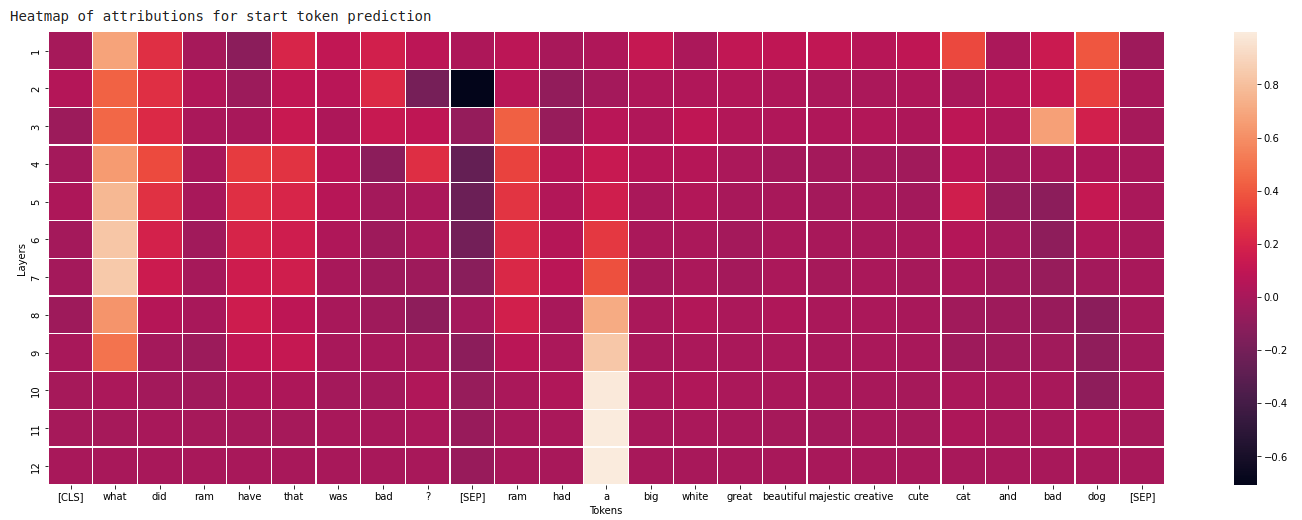
\includegraphics[scale=0.38]{Screenshot from 2022-05-02 20-32-03.png}
    \caption{Adversarial example}
    \label{obs2}
\end{figure}
\twocolumn
% \begin{figure}[!htp]
%     \centering
%     \onecolumn\includegraphics[width=\textwidth]{base_start.png}
%     \caption{}
%     \label{fig:my_label}
% \end{figure}
Clearly, the model fails here. To test heuristic 2, we constructed examples where there were no similar words or where there were more than one similar word.
\\\\Consider the context-question pairs given below \\
\textbf{Context: }Trump has a Trump card having his photo.\\
\textbf{Question: }What has Trump\'s photo?\\
\textbf{Predicted Answer: }Trump card\\
\textbf{Context: }Ram was drawing with pencils. Teacher was picking her nose with pencil. Ram observed that pencils can be used to pick nose.\\
\textbf{Question: }What was Ram's conclusion?\\
\textbf{Predicted Answer: }None\\

In the last example, if "conclusion" is replaced with "observation" in the query, the model gives correct output. This further shows the necessity of same words. This also makes the model brittle and easy to fool because there is a lack of language understanding.

To test heuristic 3, we constructed an example in which the correct answer was much farther than words on which model is focusing using heuristic one and two.\\\\Consider the context-question pair given below \ref{obs2}\\
\textbf{Context: } Ram had a big white great beautiful majestic creative cute cat and bad dog.\\
\textbf{Question: } What did Ram have that was bad?\\
\textbf{Predicted Answer: } a big white great beautiful majestic creative cute cat and bad dog \\

The heat-map for the last example shows us the full story of how the model predicts the answer. First the model focuses on "cat" and "dog" as they are candidate answers for the question word "what". The model also focuses on the word "what". Then the model finds the word "Ram" to be same in both the question and the context. Thus it focuses on "Ram" in the context. Then it looks at it's neighbouring word: "a" and predicts it for start token. The model also focuses on the word "bad" as it is also same in context and question. However, in step 4 of the heuristics, the model chooses to not "go ahead" with the word "bad". 
\section{Contributions}
\begin{enumerate}
    \item \textbf{AI20BTECH11004}: Section 2.2 in preliminary report, section 3 in mid-term report, code for captum in mid-term submission, t-SNE code in final report, minor change in bert-fine tune to save models.
    \item \textbf{AI20BTECH11006}: Section 2.1 in preliminary report, section 3 in mid-term report, code for captum in mid-term submission, t-SNE code in final report, minor change in bert-fine tune to save models.
    \item \textbf{AI20BTECH11011}: Abstract, Section 1, Conclusion in preliminary report, Section 2 in mid-term report, bert-fine-tune code in mid-term submission, Section 2.2, 2.3 in final report.
    \item \textbf{AI20BTECH11015}: Section 2.1 in preliminary report, Section 1 in mid-term report, bert-fine-tune code in mid-term submission, prepared question-ground truth dataset and , Section 2.1 in final report.
    \item \textbf{AI20BTECH11027}: Section 2.2 in preliminary report, Section 1 in mid-term report, bert-fine-tune code in mid-term submission, heat map visualization code in final-report submission, Abstract, Section 1 and 2.1 in final report.
\end{enumerate}

%%%%%%%%% REFERENCES
{\small
\bibliographystyle{ieee_fullname}
\bibliography{egbib}
}
\end{document}
